\chapter{State of the art}
\label{chap:state-of-the-art}

\section{Chatbots}
From a user point of view, chatbots are trendy nowadays, big companies such as \textit{Google} or \textit{Apple} are pushing to make the technology mainstream. Even if not every lambda people understand the word \say{chatbot}, they all have at least a mental representation of it. Indeed, they could call it Digital Assistant, Siri, Ok Google, and so on, in the end, they all understood the concept of an artificial intelligence narrowed to more or less human-like conversations.

\subsection{History of Chatbots}
When are they coming from? Not mentioning \textit{Alan Turing} or \textit{Joseph Weizenbaum}, considered as the fathers of \gls{ai} and chatbots, would not be fair. Indeed, they forecasted in 1950, that computers would be able to use human-like communication and they proposed a test to distinguish humans from machines, called the Turing Test\cite{paper:turing}. Where a human is asked to talk to a masked entity, and determine if it is talking to a human or a computer. If the human cannot determine who is the computer, then the machine passed the Turing test, as seen on figure ~\ref{fig:wikipedia_turing_test_img}. 

In 1966, Joseph Weizenbaum wrote Eliza, a computer program simulating a psychotherapist, seen as one of the first well-known attempts to make a chatbot passing Turing test. Note that due to technical restrictions, Eliza is not performing well at all time. As it is for today, it is possible to play with it at on a dedicated website. \cite{chatbot:eliza}

Since Eliza, a lot of progress has been made, indeed, to only cite a few noticeable chatbots: \textit{Parry}\cite{chatbot:parry} (1972), \textit{Jabberwack}\cite{chatbot:jabberwack} (1988), \textit{Dr. Sbaitso}\cite{chatbot:dr-sbaitso} (1991), \textit{A.L.I.C.E}\cite{chatbot:alice} (1995), \textit{Smarterchild}\cite{chatbot:smarterchild} (2001), \textit{Watson}\cite{chatbot:watson} (2006), \textit{Siri}\cite{chatbot:siri} (2010), \textit{OK Google}\cite{chatbot:google} (2012), \textit{Alexa}\cite{chatbot:alexa} (2014), \textit{Cortana}\cite{chatbot:cortana} (2014), Facebook Bots\cite{chatbot:facebook} (2016), and \textit{Tay}\cite{chatbot:tay} (2016), which where all part of the Chatbot history \cite{chatbot:futurism_history_infography}.

From IF-ELSE, \gls{aiml}, up to \gls{ml} with \gls{ann} and \gls{dnn}, the improvement in the field of chatbots increased drastically over the years. At every iteration, the algorithms are becoming more sophisticated and better at using the human language, which is now called the field of the \gls{nlp} and \gls{nlu}.

\begin{figure}[ht!]
    \centering
    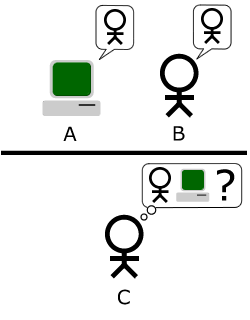
\includegraphics[width=\textwidth,height=6cm,keepaspectratio=true]{Turing_Test_version_3}
    \caption{
       The "standard interpretation" of the Turing Test, in which player C, the interrogator, is tasked with trying to determine which player - A or B - is a computer and which is a human. The interrogator is limited to only using the responses to written questions in order to make the determination. \cite{wikipedia:turing_test_img}
    }
    \label{fig:wikipedia_turing_test_img}
\end{figure}

\subsection{Narrow Chatbots}
Once again, chatbots are almost everywhere nowadays. Indeed, it became a common tool for companies of any size to communicate with their customers and a toy for users. However, most of the time, Chatbots are not understood by their users and is leading to a high level of frustration. Even if they are becoming increasingly mainstream and sophistical, people do not realize their limits. Today's chatbots are often mistaken for \gls{agi} in \gls{scifi} and are expected to do much more than they can do. Indeed, making \gls{ani} chatbots implies a specialization into a specific field.

Not to forget that the primary purpose of chatbots is to provide a conversational service to the user from text to vocal or even visual format. However, its purpose can derivated in an almost unlimited amount of solutions such as Health, Weather, Customer Service, Games, and much more.

\subsection{\gls{ir} Chatbots}
Most of the time used by \gls{faq} chatbots, which are probably the most common type of chatbots, its goal is to answer specific questions, based on a specific keyword. Indeed, the communication skills are limited to pre-made sentences and a question/answer database, which often results in the best case scenario in a perfect match, or the worst case scenario would be the return of something unexpected.

Technically speaking, \gls{ir} is part of the \gls{dm} in the field of \gls{ml}. It is well suited for search engines, as it works in a query mode. Indeed, the algorithm tries to find the best match to the submitted query in its database, usually with pattern extraction and a rank. 

\subsection{Sequential Chatbots}
\say{If he says this, then say that, then do so.}
This sentence is a good example of the concept of sequential chatbots. From a communication point of view, it does not have to talk to accomplish its purpose; it is indeed usually based on a keyword detection technic to determine what pre-made action to do. However, as the whole system works on pre-made actions, the development of such algorithms requires a lot of brain power from the developers. Indeed, as all actions result from anticipated specific keywords, and even specific order of keywords, the complexity can quickly increase, which most of the time, makes sequential chatbots seen as command line terminals instead of conversational chatbots.

\subsection{Forwarding Chatbots}
Often used by companies for customer service, it has become the most popular type of chatbots and seen as a hybridization of the \gls{ir} and sequential chatbots. Its goal is to simulate an agent that is available 24/7 to help the customer. Indeed, it will try its best to answer the most popular questions based on its \gls{faq} database and forward the user seamlessly to a human agent if its knowledge is getting limited. In the best case scenario, it is greatly appreciated by the user as the transition from chatbot to human is not noticeable.

\subsection{Learning Chatbots} 
As \gls{ml} evolves at an incredible rate and boosted by \gls{dnn}, new \gls{nlp} algorithms emerges, and most of the time leaves the previous generation far behind. Modern learning chatbots algorithms are what comes closer to human-like conversations. Leaving the algorithm alone progress through iterations on a large dataset or commonly named \gls{bd} of real conversations, it will learn patterns by itself. However, the output generated by the trained model is dependent on the data the training occurred on. The most well-known example is \textit{Tay}\cite{chatbot:tay} (2016), the Twitter chatbot from Microsoft, that was influenced by the 4chan community to make it speak like a Young Racist Girl.
However, it is essential to take note that learning chatbots are exciting for a long time now. \textit{A.L.I.C.E}\cite{chatbot:alice} had already basic learning skills, as \gls{aiml} was taking care of saving variable on the run, such as the first name of the user. Even if this methodology could be seen archaic if compared to new \gls{dl} algorithms such as LSTM, it is still used today likewise the \gls{aiml} technology.


\subsection{Proactive Chatbots}
\say{Hey, I saw that you are on the website for some minutes now, do you need some more dedicated information?}. It is almost impossible that someone never received a message alike. Indeed, proactivity is not new in the field of chatbots, mimicking an interest from the chatbot to initiate conversations has become a standard in marketing and customer support chatbots. However, the limitations are hit fast, beyond asking general questions, not much progress has been made until now.

True proactive chatbots are implying that the algorithm is capable of initiating conversations from a human-like perspective, initiating the conversation or asking information in a meaningful manner based on the user, the context and the relationship with the user. The state-of-the-art search could not find any evidence of existing real proactive chatbots as described.


\subsection{Chatbot Examples}
As a help to get a feeling about narrow chatbots, a none-exhaustive list of applications is available below, and for more references about chatbots, Chatbot.org\cite{chatbot:chatbots-org} is an excellent, up to date, place about referencing old and new chatbots.

\begin{itemize}
\setlength\itemsep{0em}
\item Receive relevant information about a trip, book flights, and hotels, and get updated on the boarding and weather conditions at the airport.
\item Keep track and order coffee remotely at the office.
\item Monitor customer's satisfaction.
\item Convert potential customer into paying customers by interacting with them at the right moment.
\item Personal assistant on-the-go, get the schedule and the next meetings.
\item Relay for people on hold at a service.
\end{itemize}


\subsection{Narrow Chatbots compared to General Chatbots}
Before going further into the world of general chatbots, it is required to understand the following two axes of \gls{ai} defined by Tasks and Knowledge.
Indeed, narrow chatbots are limited by the range of tasks they can accomplish and the knowledge they can use. However, most of the time, they are very good at a particular task for a particular knowledge requirement. The table \ref{tab:agi-ani-gc} tries to represent the position of Narrow and General Chatbots on those two axes.

\vspace{1em}
\textbf{Tasks:}
Talk, \gls{faq}, Remote Control, Customer, or Placing orders are just a few tasks that a chatbot could accomplish.

\vspace{1em}
\textbf{Knowledge:}
Health, Weather, Customer Service, or Games are just a few knowledge examples chatbots could excel at.

\newcommand\MyBox[2]{
  \fbox{\lower0.75cm
    \vbox to 2cm{\vfil
      \hbox to 6cm{\hfil\parbox{5cm}{#1\\#2}\hfil}
      \vfil}
  }
}
%\noindent
%\renewcommand\arraystretch{1.5}
\setlength\tabcolsep{0pt}
\begin{table}[H]
\centering
\begin{tabular}{c >{\bfseries}r @{\hspace{0.7em}}c @{\hspace{0.4em}}c @{\hspace{0.7em}}l}
  \multirow{10}{*}{\rotatebox{90}{\parbox{5.5cm}{\bfseries\centering Tasks}}} & 
  & \multicolumn{2}{c}{\bfseries Knowledge} & \\
  & & \MyBox{Expert in a specific Field}{Expert at all Tasks} & \MyBox{\textbf{General Chatbots}\\Expert in all Fields}{Expert at all Tasks} \\[2.4em]
  & & \MyBox{\textbf{Narrow Chatbots}\\Expert in a specific Field}{Expert at specific Task} & \MyBox{Expert in all Fields}{Expert at specific Task} \\
\end{tabular}
\caption{Tasks versus Knowledge in the field of Chatbots}
\label{tab:agi-ani-gc}
\end{table}



%\begin{minipage}{\textwidth}
\subsection{General Chatbots}
Much effort is being made to get chatbots able to perform well simultaneously in various tasks and knowledge. Indeed, general chatbots should are not limited to previously learned tasks and subjects; they should also be able to learn and relearn. 
Those type of chatbots have not been found during the state of the art phase, and are probably by this mean either none-existant at the moment or hidden in laboratories, far from public knowledge. 
However, big companies like Amazon are providing to the public a feel of general chatbots with \textit{Alexa}\cite{chatbot:alexa}. Users can converse with it, command their smart houses, use it as a personal assistant, and even program it to perform custom actions. However, it is not yet able to learn by itself and generate out of the blue none-programmed skills.
Note that general chatbots could be scary for lambda people if it starts mimicking human being too well, as in the user mind, talking to a machine should be differentiable from talking to humans. Admittedly, in the case of the \textit{Turing Test}\cite{paper:turing}, the human does not know if it is talking to a human or a machine, which makes it probably more comfortable to accept than talking to a machine directly. \gls{scifi} is conditioning people to believe that human-like performing machines are dangerous for the human species.


\subsection{From \gls{ani} to \gls{agi}}
On a side, even if it is not part of the deepening project. It is interesting to write a few lines about \gls{ai}. New incredible algorithms outperforming the previous one, and experiments reports are emerging almost every month and redefining the standard of \gls{ai}. Paradigms are shifting and technologically speaking; we are entering a new era of computer-assisted humankind.

\subsection{\gls{ani}}
More than a sequential algorithm, narrow artificial intelligence in modern terminology is the definition of \say{being good at something}. \gls{ani} has been made possible with the huge progress in \gls{ml}, the arrival of the \gls{dl}, and the need for humans to store data about everything (\gls{bd}). In medicine, for instance, it is sometimes performing so well, that humans, who spent years studying are left behind by an algorithm trained large datasets for a few days.

\subsection{\gls{agi}}
The next step into the field of \gls{ai}, when supervision has been banned as a teaching method for algorithms as the human interaction is inputting more errors than machine themselves if unsupervised. In addition to teaching themselves, algorithms are teaching each other, and improve over the iteration with auto corrections and optimizations. They are excelling at all tasks requiring repetition, precision, and safety. Besides, they are also all able to retrieve any available information and use it for their need. \say{In the future, machines will be able to understand and do everything, much more efficiently than humans.}
%\end{minipage}

\section{Word2Vec}
\subsection{What is Word2Vec}
\subsection{Gensim}
\subsection{Framworks}


\section{Word Embedding Alternatives}
\subsection{FastText}
\subsection{Glove}
\subsection{Word2Vec-f}
\subsection{Wang2vec}


\section{Sentence/Document Embedding Alternatives}
\subsection{Doc2vec}
\subsection{Skip-thought}
\subsection{Smooth Inverse Frequency}
\subsection{RNN}


\section{Datasets}

% figures
%h (here) - same location
%t (top) - top of page
%b (bottom) - bottom of page
%p (page) - on an extra page
%! (override) - will force the specified location

